\documentclass[12pt]{article}
\usepackage[paper=a4paper,left=30mm,right=30mm,top=35mm,bottom =35mm]{geometry}
\usepackage[utf8]{inputenc}
\usepackage[T1]{fontenc}
\usepackage{stmaryrd}
\usepackage{setspace}
\usepackage{mathrsfs}
\usepackage[ngerman]{babel}
\usepackage{amssymb}
\usepackage{amsmath}
\usepackage{fancyhdr}
\usepackage[dvips,unicode,colorlinks,linkcolor=black]{hyperref} 
\usepackage{graphicx}
\usepackage{float}

\pagestyle{fancy}
\lfoot{}
\rfoot{Paul Kremser, Tobias Grussenmeyer}
\cfoot{\thepage}
\fancyhead[L]{FPI Versuch: Kernspin}
\renewcommand{\headrulewidth}{0.6pt}
\renewcommand{\footrulewidth}{0.6pt}
\setlength{\headheight}{16pt}
\setlength{\parindent}{0pt}
% Für die Wahl der Schriftart
\newcommand{\changefont}[3]{
\fontfamily{#1} \fontseries{#2} \fontshape{#3} \selectfont}

\begin{document}
% keine Hurenkinder und Schusterjungen
\clubpenalty = 10000
\widowpenalty = 10000 
\displaywidowpenalty = 10000

\onehalfspacing
% Schriftart
\changefont{ptm}{m}{n} 

\begin{titlepage}
\author{Paul Kremser, Tobias Grussenmeyer}
\title{Versuch: Kernspin}
\date{Versuchsdurchführung: 12. November 2009} 
\maketitle
\thispagestyle{empty}
\end{titlepage}


\tableofcontents
\thispagestyle{empty}
\newpage
\pagenumbering{arabic}
\section{Überblick}

\section{Aufgabestellung}
\begin{itemize}
 \item Bestimmung des Magnetfelds des Permantentmagneten, Untersuchung der Homogenität.
 \item Bestimmung des gyromagnetischen Verhältnis des Protons in einer Glykolprobe
 \item Untersuchung der Protonenresonanz einer Wassersotffprobe
 \item Bestimmung des kernmagnetischen Moments des $^{19}F$-Kerns in einer Teflonprobe
 \item Wiederholte Messung einer Probe mit der Lock-in Methode (Synchrondetektor)
\end{itemize}


\section{Theoretische Grundlagen}

\subsection{Spin}
Der Spin ist eine quantenmechanische Eigenschaft von Elementarteilchen, eine Art von nicht-klassischer Eigenrotation. Weil aber die zugehörige klassische Vorstellung nach heutiger und logischer Sichtweise falsch ist, kann der zuletzt benutzte Begriff beim Verständnis nur bedingt behilflich sein. Der Spin verhält sich mathematisch bis zu gewissem Grade als Drehimpuls. Der Erhaltungssatz des Gesamtdrehimpulses gilt allerdings nur für die Summe aus (klassischem) Bahndrehimpuls und Spin eines Systems. Daher ist der Spin im Gegensatz zum Isospin nicht nur mathematisch eine dem Bahndrehimpuls analoge Eigenschaft, sondern tatsächlich eine Art von Drehimpuls, allerdings von Anfang an ein nicht-klassisches Phänomen.\\

In einem Magnetfeld kann der Spin $\vec{J}$ nur diskrete Werte annehmen
\begin{align}
 J_s = \hbar \cdot m_{I}
\end{align}

$m_I$ kann ganzzahlige oder halbzahlige Werte $-I, -I+1, -I+2, ..., I-1, I$ annehmen. Insgesamt gibt es $2I+1$ mögliche Einstellmöglichkeiten. Bei Protonen und auch bei dem $^19 F$-Kern ist $I = \frac{1}{2}$. Es gibt somit nur die beiden Einstellmöglichkeiten $m_i = \pm \frac{1}{2}$. Der Spin kann sich parallel oder antiparallel zum Magnetfeld ausrichten.

\subsection{Magnetisches Moment}
Fasst man den Spin als Rotation eines geladenen Elementarteilchens auf so entsteht ein magnetisches Dipolmoment. Dieses Dipolmoment ist proportional zum Spin. Beschränkt auf dei $z$-Komponente, gilt:
\begin{align}
 \mu_z = g_K \cdot \mu_K \cdot m_I
\end{align}

Bei Spin Null resultiert kein magnetisches Dipolmoment. Der Betrag von $\vec\mu$ wird vom Kernmagneton $\mu_K$ bestimmt. $g_K$ hängt vom jeweiligen Kern ab.
\begin{align}
 \mu_K = \frac{e \cdot \hbar}{2 \cdot \mu_p} = 5,05079 \cdot 10^{-27} J \cdot T^{-1}
\end{align}

\subsection{Spin im Magnetfeld}
Legt man das Magnetfeld in $z$-Richtung an so wird die potentielle Energie $E_{pot} = -\vec\mu \cdot \vec B$ zu:
\begin{align}
 E_{pot} = -g_K \cdot \mu_K \cdot m_I \cdot B_z
\end{align}

Für Spin $\frac{1}{2}$ Teilchen erhält man zwei unterschiedliche Energieniveaus mit Abstand:
\begin{align}
 \Delta E = g_K \cdot \mu_K \cdot B_z
\end{align}

Genau diese Energie wird benötigt bzw frei wenn der Spin im Magnetfeld zwischen beiden Niveaus umklappt.

\subsection{Resonanz}
Bei Einstrahlung elektromagnetischer Strahlung kann, wenn die Energie gerade dem energetischen Abstand $\Delta E$ der beiden Spin Nieveaus entspricht, das Umklappen der Spins angeregt werden. Stimmt die Frequenz so klappen die Spins im energetisch tieferen Niveau in das höhere Niveau um und entziehen dem elektrischen Feld somit Energie. Allerdings bewirkt die Stahlung auch das umgekehrte Umklappen wobei Energie and das Stahlungsfeld abgegeben wird. Hierbei spricht man von der induzierten Emission. Die jeweilige Wahrscheinlichkeit für Absorption bzw. Emission ist proportional zur jeweiligen Besetung der Spinzustände.\\

Laut Bolzmann befinden sich im thermischen Gleichgewicht mehr Spins im energetisch tieferen Zustand:
\begin{align}
 \frac{n_{high}}{n_{low}} = e^{-\frac{g_K \mu_K B_z}{k_B T}} 
\end{align}

Für Protonen und das im Versuch vorliegende Magnetfeld ergibt sich ein Besetzungsunterschied von $3\cdot 10^{-6}$, was in einer makroskopischen Probe immer noch etwa $10^{17}$ Teilchen mehr im tieferen Zustand bedeutet. Letztendlich ist es also insgesamt möglich dem Strahlungsfeld Energie zu entziehen. Dies lässt sich als Form von Dämpfung im Schwingkreis beobachten.

\subsection{Relaxation}
Logischerweise stellt sich nach kurzer Zeit der Anregung ein Gleichgewicht zwischen den beiden Spinzuständen ein.
Somit müsste die Dämpfung des Feldes schon nach kurzer Zeit wieder zum Erliegen kommen. Jedoch gibt es noch weitere Prozesse welche an dem Vorgang beteiligt sind. In erster Linie zählen hierzu die \textbf{Spin-Gitter-Relaxation} und die \textbf{Spin-Spin-Relaxation}. Bei der Spin-Gitter-Relaxation geht Energie aus dem Spinsystem in Gitterschwingungen über. Hierbei wird praktischerweise keine Strahlung abgegeben, die Energie aus dem Stahlungsfeld geht schlicht in Wärme über. Die Spin-Gitter-Realaxation versucht also die Situation gemäß der Bolzmanstatistik wieder herzustellen. Die Spin-Spin-Relaxation kommt durch Wechselwikung magnetischer Momente untereinander zustande und führt im wesentlichen zu einer Verbreiterung der Absorptionslinie.\\

Die Relaxationen brauchen selbstverständlich Zeit, die sogenannte Relaxationszeit. Bei den im Versuch verwendeten Proben sind diese aber noch viel zu lang ist um auszureichen eine Messbare Dämpfung des Systems zu produzieren. Durch Zusatzt paramagnetischer Ionen können die Relaxationszeiten um Größenordnungen reduziert werden. In unserem Versuch wird dazu $Mn(NO_3)_2 + 4H_2O$ verwendet.

\subsection{Synkrondetektor}


\section{Versuchsaufbau}
Das für den Versuch benötigte starke Magnetfeld wird von einem Permanentmagneten erzeugt. Über zwei an den Polschuhen angebrachte Spulen kann eine kleine Änderung des Permanentfelds erzeugt werden. Mittels eines Addierers können von verschiendenen Generatoren stammende Spannungsverläufe auf die Spulen gegeben werden (Sinusspannung, Sägezahn).\\

Auf einem Schlitten befindet sich die Elektronik an welche die Probe angeschlossen wird. Die Probe lässt sich sowohl horizontal als auch vertikal verschieben und somit optimal zwischen den Polschuhen des Permanentmagneten plazieren.
Die Proben sind von einer Schwingkreisspule umgeben über welche ein hochfrequentes Feld eingestrahlt wird. Über die Elektronik wird ein niederfrequentes Signal ausgekoppelt welches auf dem Oszilloskop beobachtet werden kann.

\section{Durchführung}

\section{Auswertung}
\begin{figure}[H]
\centering
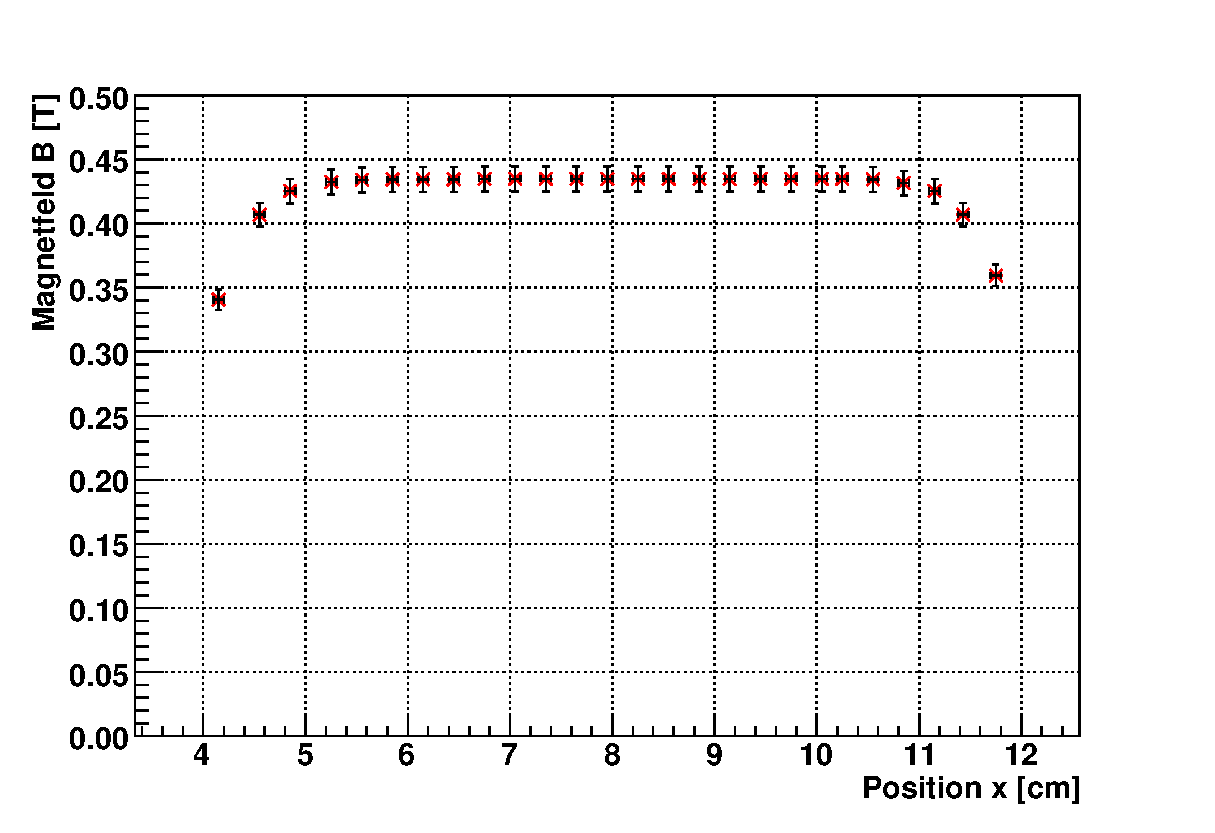
\includegraphics[width=0.9\linewidth]{pictures/hallsonde_x.eps}
\caption{Magnetfeldmessung mit Hallsonde x-Richtung}
\end{figure}

\begin{figure}[H]
\centering
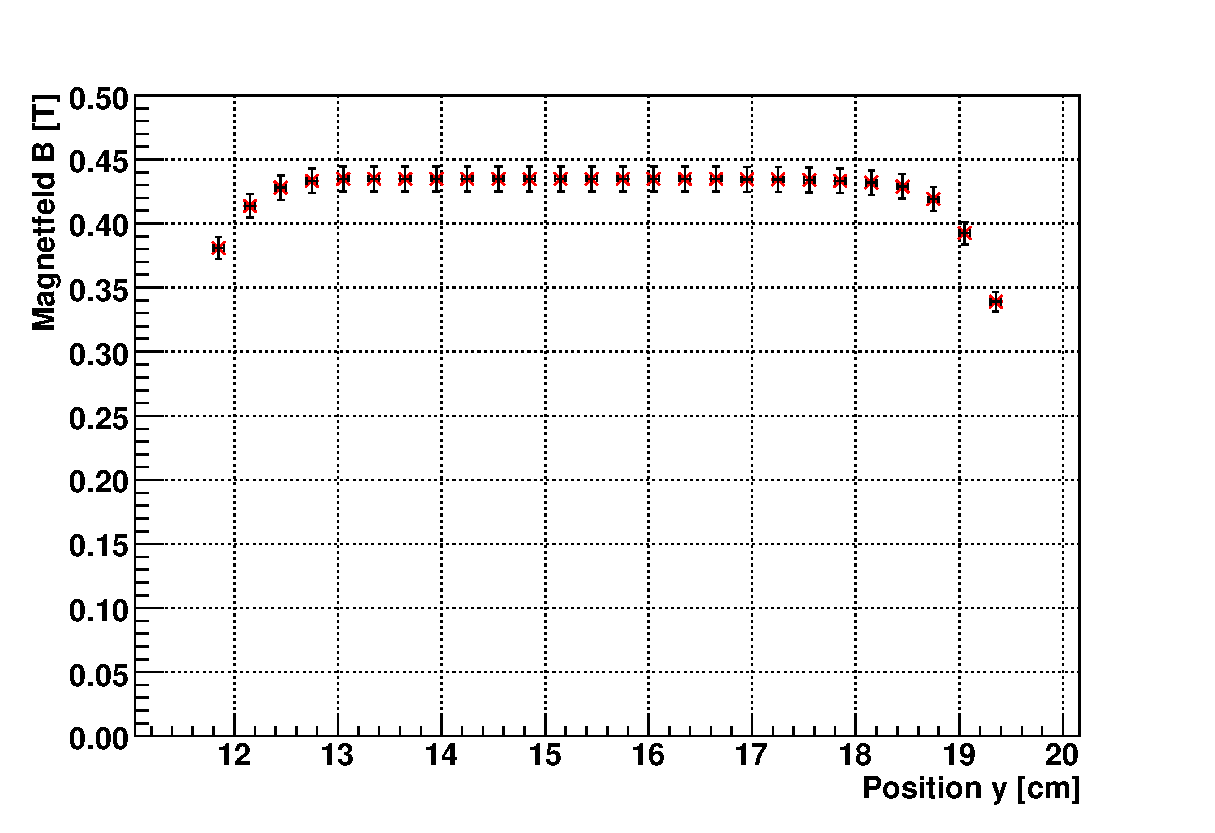
\includegraphics[width=0.9\linewidth]{pictures/hallsonde_y.eps}
\caption{Magnetfeldmessung mit Hallsonde y-Richtung}
\end{figure}

\begin{figure}[H]
\centering
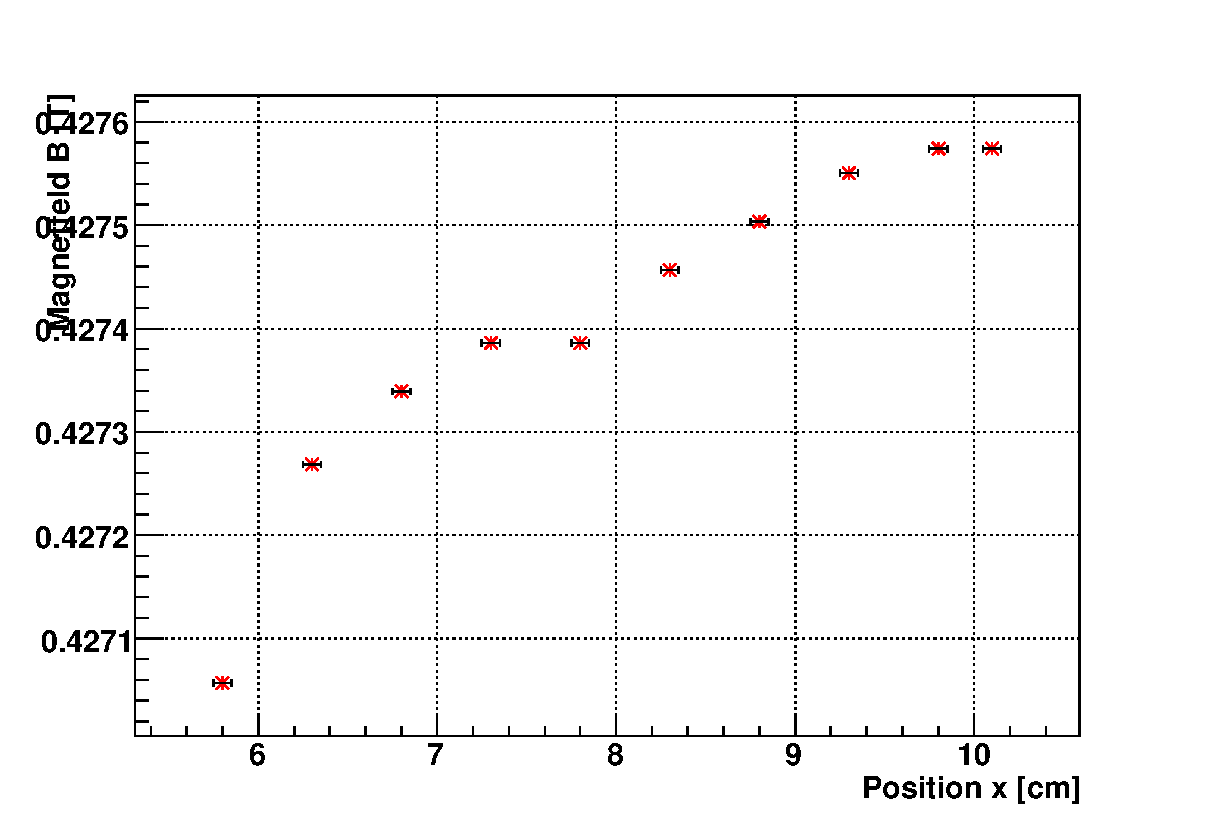
\includegraphics[width=0.9\linewidth]{pictures/wasser_x.eps}
\caption{Wasserstoffprobe x-Richtung}
\end{figure}

\begin{figure}[H]
\centering
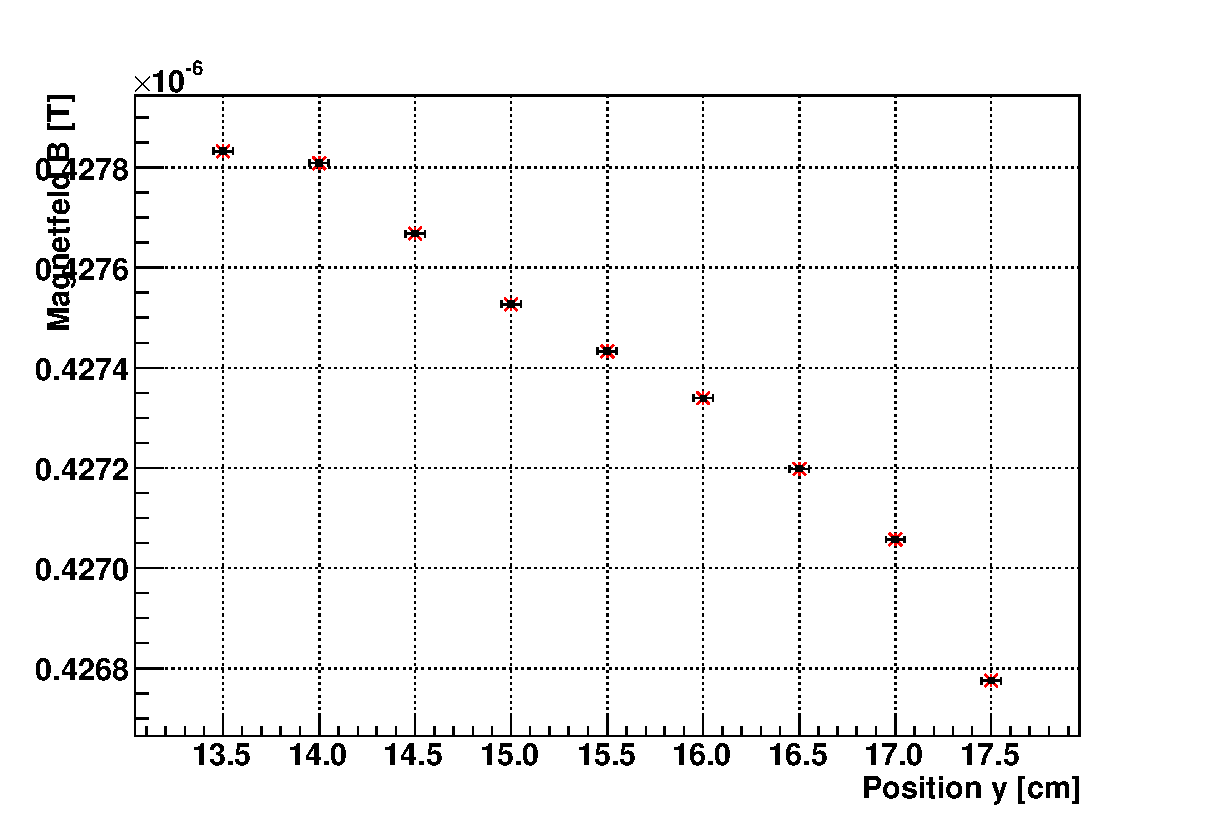
\includegraphics[width=0.9\linewidth]{pictures/wasser_y.eps}
\caption{Wasserstoffprobe y-Richtung}
\end{figure}



\section{Zusammenfassung}

\end{document}
